\thispagestyle{lichsutoanhocnone}
\pagestyle{lichsutoanhoc}
\graphicspath{{../lichsutoanhoc/pic2/}}
\everymath{\color{lichsutoanhoc}}
\blfootnote{$^1$\color{lichsutoanhoc}THPT chuyên Hà Nội -- Amsterdam.}
\begingroup
\AddToShipoutPicture*{\put(0,616){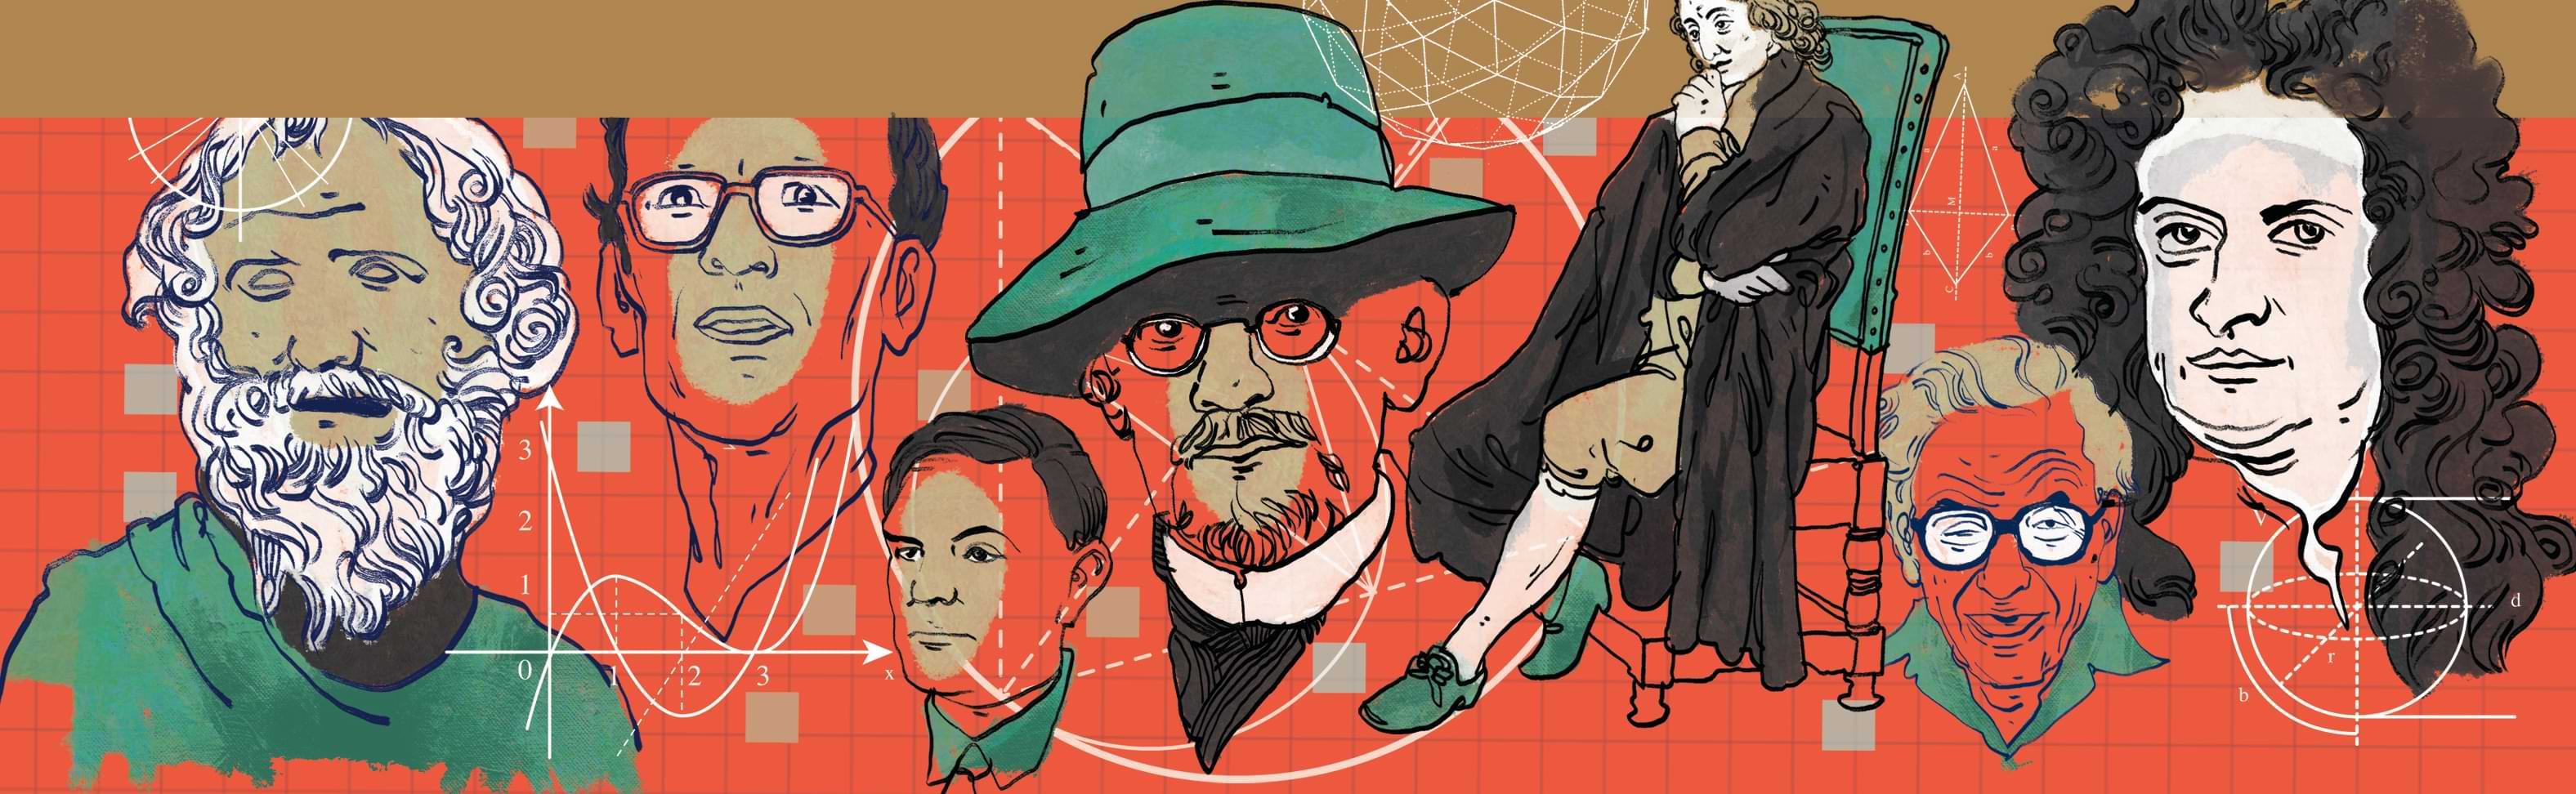
\includegraphics[width=19.3cm]{../bannerlichsu}}}
\AddToShipoutPicture*{\put(82,555){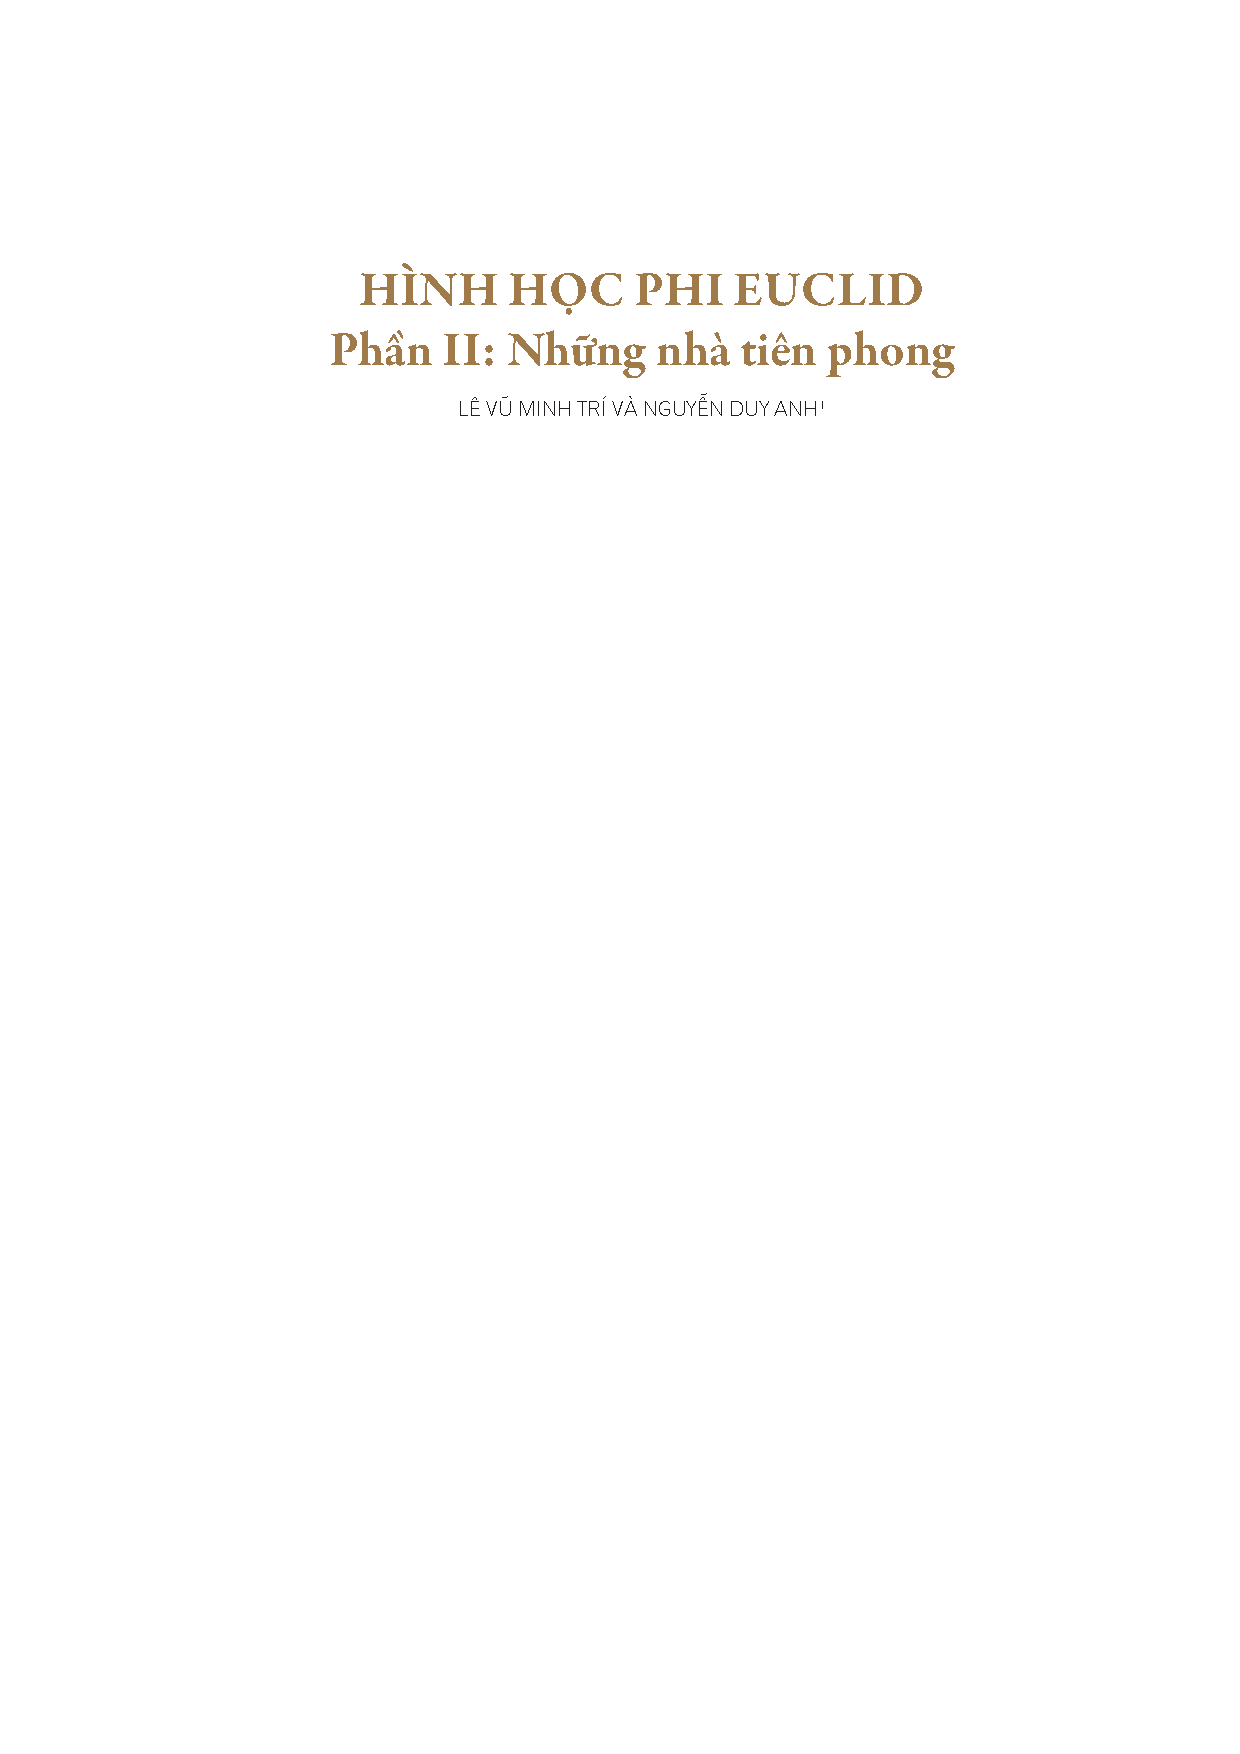
\includegraphics[scale=1]{../tieude3.pdf}}}
\centering
\endgroup

\textbf{Hiệp: sửa tiêu đề thành}

{Hình học phi Euclid\\
Phần III: Kiểm chứng sự tồn tại}

Trong phần còn lại của hành trình, chúng ta sẽ cùng đi qua một chứng minh cho định lý quan trọng nhất khẳng định sự ``đúng đắn'' của vũ trụ mới - hình học hyperbolic:

Định lý toán học siêu hình
\footnote{Metamathematics: bộ môn nghiên cứu về toán học bằng các phương pháp toán học, chẳng hạn như liệu một hệ tiên đề có chứa mâu thuẫn nào không.}: \textit{Nếu các tiên đề của hình học Euclid không dẫn tới mâu thuẫn nào, thì các tiên đề của hình học hyperbolic cũng vậy. }



Để có thể đào sâu vào hai vũ trụ hình học hyperbolic và elliptic khác biệt đến vậy, chúng ta buộc phải truy ngược về những điều căn bản nhất - các tiên đề. Tất nhiên, chúng tôi sẽ cố gắng để bài báo vẫn giữ được nét đẹp từ việc nhìn và cảm nhận các hình vẽ như ở hình Euclid. Suy cho cùng, các tiên đề ban đầu lập ra chính là để đảm bảo ghi lại được những cảm nhận đó bằng logic. 

Hy vọng rằng qua đây, độc giả thấy được sự quen thuộc của hai thế giới phi Euclid tưởng xa lạ, và có một cái nhìn mới mẻ hơn về hình học Euclid, quê hương thân thuộc của ta.

\section{Tiên đề của hình học Euclid}

Khi nền toán học phát triển và logic chặt chẽ hơn, con người dần hiểu ra rằng một chứng minh phụ thuộc vào hình vẽ và các ngộ nhận sẽ không chính xác. Năm tiên đề của Euclid đưa ra, được ca tụng là đỉnh cao chặt chẽ suốt hai thiên nhiên kỷ còn là quá ít. Chúng ta có thể bóc tách một vài chứng minh của Euclid để nhận ra những gì còn thiếu, và trong quá trình đó đặt ra hình học Euclid cần tới những tiên đề nào. 

Tiết toán đầu tiên của năm lớp Sáu,  chúng ta  được học thế nào là tập hợp: nó là một khái niệm nguyên thủy, sẽ không có định nghĩa. Muốn định nghĩa tập hợp là gì thì học sinh sẽ phải biết một khái niệm cơ bản hơn từ trước, và như thế thì phải có tiết nào đó trước tiết về tập hợp để nói về nó, cứ như vậy thì lùi mãi, làm sao năm học có thể bắt đầu! Một trong các sai lầm Euclid mắc phải chính là cố định nghĩa hết các khái niệm cơ bản như đường thẳng và điểm.
	
	
	 
	\vskip 0.1cm

	Ta cùng nhìn vào vài ví dụ từ Elements để chỉ ra các thiếu sót của Euclid. 
	\vskip 0.1cm
	Định lý $1$: Luôn tồn tại một tam giác đều các cạnh dài bằng $AB$ với mỗi đoạn $AB$ cho trước 
	\vskip 0.1cm
	Chứng minh của Euclid: Theo Tiên đề $3$, ta vẽ được đường tròn tâm $A$ bán kính $AB$ và đường tròn tâm $B$ bán kính $BA$. Nối cạnh từ một giao điểm $C$ nào đó của hai đường tròn tới $A$ và $B$ thì $AC = AB$ và $BC = BA$ theo định nghĩa đường tròn, từ đó theo định đề $1$ thì tam giác $ABC$ là tam giác đều.
	\vskip 0.1cm
Euclid ở đây đã không để ý đến việc chứng minh sự tồn tại của giao điểm C, năm
tiên đề ông đưa ra cũng không đủ để chứng minh điều này. Ngoài ``nhìn hình ta có'', có thể hiểu một cách trực quan là hai đường tròn phải ``liên tục'' nên sẽ cắt nhau. Hệ thống tiên đề lại chưa nói gì về điều này, nên cách giải quyết duy nhất là thêm một tiên đề mới. Một giải pháp khả dĩ là một tiên đề về ``tính liên tục'':	
	\vskip 0.1cm
	Nếu một đường thẳng/đường tròn chứa trên nó một điểm trong và một điểm ngoài một đường tròn khác, hai đối tượng sẽ có hai giao điểm.
	\vskip 0.1cm
	Hay Định lý $4$, trường hợp bằng nhau cạnh--góc--cạnh: Với hai tam giác $ABC$ và $A'B'C'$ có $AB = A'B'$, $AC = A'C'$, $BAC = B'A'C'$, ta dịch chuyển tam giác $ABC$ sao cho $A$ trùng $A'$ và cạnh $AB$ được đặt lên $A'B'$. Do $AB = A'B'$ nên $B$ trùng $B'$, và do góc $A =$ góc $A'$, $AC$ và $A'C'$ cùng hướng, hai cạnh lại bằng nhau nên $C$ trùng $C'$ nốt. Hai tam giác trùng khớp hoàn toàn, nên chúng bằng nhau.
	\vskip 0.1cm
	Ở đây ta lại thấy xuất hiện sự ``dịch chuyển'' vốn không được quy định ở đâu trong năm tiên đề, và Euclid ngầm cho rằng sau quá trình ``dịch chuyển'' này thì tam giác $ABC$ vẫn giữ nguyên tính chất vốn có. Để tránh phiền phức, tiêu chuẩn bằng nhau này của tam giác đã được cho làm một tiên đề về quan hệ ``bằng nhau''.
	\vskip 0.1cm
	Ngoài hai mảng lớn trên, chúng ta còn phải quy định thêm về quan hệ ``nằm trên/đi qua'' (incidence) của điểm và đường thẳng, quan hệ ``nằm giữa'' (betweenness), và quan hệ ``song song'' (parallelism), vấn đề chính của ta. 
	Chúng ta cùng thử xây dựng một vài tiên đề cho quan hệ ``nằm trên/ đi qua'' (NTĐQ)
	\vskip 0.1cm
	Ta bắt đầu với bốn khái niệm nguyên thủy: điểm, đường, quan hệ nằm trên và quan hệ đi qua qua, và các tiên đề sau:
	\vskip 0.1cm
	$0.$ Điểm $P$ nằm trên đường thẳng $l \Leftrightarrow$ Đường thẳng $l$ đi qua điểm $P$
	\vskip 0.1cm
	$1.$ Với hai điểm $P$, $Q$ phân biệt bất kỳ, tồn tại đúng $1$ đường thẳng đi qua cả $P$ và $Q$. Đây là tiên đề $1$ của Euclid.
	\vskip 0.1cm
	$2.$ Có ít nhất hai điểm phân biệt nằm trên một đường thẳng $l$ bất kỳ. Một sự thật nho nhỏ là khác với chúng ta ngày nay, có vẻ như người Hy Lạp cổ đại không nghĩ về đường thẳng như được cấu thành từ các điểm. Thế mới thấy, lần nữa, có những mệnh đề đôi khi ta quên mất là mình ngầm thừa nhận, do đó cần phải phát biểu đầy đủ các tiên đề.
	\vskip 0.1cm
	$3.$ Tồn tại ba điểm phân biệt sao cho không có đường thẳng nào đi qua đồng thời cả ba điểm này. Điều này đảm bảo sự tồn tại của tam giác trên mặt phẳng hình Euclid. Một ví dụ thỏa mãn cho thấy sự cần thiết chính là một đường thẳng và các điểm nằm trên đó: cấu trúc này vẫn cứ thỏa mãn những tiên đề trên, và những tam giác vuông hay đường tròn lại không hề tồn tại ở đây.
	\vskip 0.1cm
	
\section{Ví dụ cho mô hình}
	Để minh họa cho những gì vừa thiết lập, chúng ta sẽ xét những ``mô hình'' của hệ tiên đề này. Một mô hình hiểu nôm na là một cách gán các khái niệm nguyên thủy và các quan hệ cơ bản với các đối tượng cho sẵn, sao cho các tiên đề là các mệnh đề đúng trong hệ thống đối tượng đó. Nghe có hơi trừu tượng, nên sau đây là số một ví dụ.
	\vskip 0.1cm
 Xét ba nhà Toán học là Gauss, Bolyai, và Lobachevsky. Mỗi người ta hiểu là một ``điểm'', và mỗi ``đường'' là một cặp nhà toán học có nghiên cứu về hình học phi Euclid. Một điểm được gọi là nằm trên một đường nếu trong cặp nhà toán học có chứa người đó. Đây chính là một mô hình của những gì ta vừa thiết lập.
	\vskip 0.1cm
	Điều chúng ta vừa làm nghe hơi kỳ, do cách hiểu điểm và đường thẳng này là khác với thông thường. Nhưng nhớ rằng chúng là các khái niệm nguyên thủy, điều cần quan tâm duy nhất khi nhìn nhận ``điểm'' và ``đường thẳng'' dưới con mắt logic là cách chúng vận hành. Và ở đây không khó để kiểm tra rằng thiết lập như trên thỏa mãn các tiên đề đã đặt ra. Với những ai có một số kiến thức cơ bản về lý thuyết đồ thị, bài toán với các đối tượng như ``người'' -- ''quen nhau'', ``thành phố'' -- ``có đường bay giữa hai nơi'', ``bạn bè'' -- ``ngồi cạnh nhau'' có thể coi là những mô hình cho các kết quả về ``điểm'' -- ''cạnh'' của đồ thị. 
	\vskip 0.1cm
	Quay lại với mô hình ba ``điểm'' vừa dựng, có một tính chất hiển nhiên là hai đường thẳng bất kỳ trong mô hình đều có giao điểm. Một cách không khó hiểu, ta gọi một mô hình như thế này là có tính chất elliptic.
	\vskip 0.1cm
	Và bởi không có tính chất nào trong số các tiên đề ta vừa nêu nói rằng đường thẳng phải ``dài'', ta hoàn toàn có thể xét mô hình như sau và có các kết quả tương tự: quy ước các ``điểm'' là các cặp nhà toán học \{Gauss, Bolyai\}, \{Bolyai, Lobachevsky\}, \{Lobachevsky, Gauss\} và các ``đường thẳng'' là Lobachevsky, Gauss và Bolyai. Một điểm $P$ được gọi là nằm trên một đường thẳng $d$ nếu cặp nhà toán học biểu diễn $P$ chứa nhà toán học đại diện cho $d$. 
	\vskip 0.1cm
	Với mô hình với bốn điểm $A$, $B$, $C$, $D$, hai điểm đôi một có một đường thẳng đi qua, tiên đề song song của Euclid lại đúng, ví thử như với đường thẳng qua $A$, $B$, điểm $C$, thì có đúng một đường $CD$ là đi qua $C$ và song song $AB$, ta gọi mô hình như vậy là có tính chất Euclid. Với năm điểm $A$, $B$, $C$, $D$, $E$, mô hình lại thỏa mãn tính chất hyperbolic: chẳng hạn với cạnh $AB$ và điểm $C$ thì có $CD$, $CE$ song song (không có giao điểm) với $AB$ (lưu ý toàn bộ các điểm ở đây ta xét chỉ gồm $A$, $B$, $C$, $D$, $E$, nếu vẽ trên giấy mà các đường thẳng có giao nhau tại một điểm không thuộc năm điểm kia, ta không tính).
	\vskip 0.1cm
Như vậy, chúng ta đã thấy những ví dụ chứng tỏ rằng hình học với những tính chất phi Euclid phần nào có tồn tại, và thật ra, không có gì khó hiểu cả. Tuy nhiên, ta mới chỉ dựng ra được những mô hình thỏa mãn các tiên đề nằm trên/đi qua, một góc nhỏ của hình học Euclid. Hãy cùng đến với một ví dụ gần với hình Euclid hơn nữa

\section{Từ tỷ số kép tới một nửa địa cầu}
Dù hình học phi Euclid ban đầu hiện lên xa lạ với cảm nhận của con người, ta có thể tiếp cận nó ngay từ những ý tưởng trong chính hình học Euclid chúng ta được làm quen ngay từ trung học cơ sở. Trước tiên ta nhắc lại một khái niệm quen thuộc với những người học hình Euclid -- tỷ số đơn, tỷ số kép.
	\vskip 0.1cm
	Cho ba điểm $A$, $B$, $C$ thẳng hàng và đôi một phân biệt, tỷ số đơn $(AB, C)$ là số thực $ \dfrac{\overline{CA}}{\overline{CB}}$, có giá trị tuyệt đối bằng $\dfrac{CA}{CB}$, mang dấu âm nếu $ \vec{CA}, \vec{CB}$ ngược hướng, tức là khi $C$ nằm giữa $A$ và $B$, và mang dấu dương trong các trường hợp còn lại. 
	\vskip 0.1cm
	Xét thêm điểm $D$ trên cùng đường thẳng với ba điểm trên, định nghĩa tỷ số kép $(AB, CD)$ là:
	$(AB, CD) = (AB, C) : (AB, D)$
	Phép chiếu xuyên tâm được định nghĩa là: với hai đường thẳng $d$, $d'$ và một điểm $P$ không nằm trên chúng. Khi ấy phép chiếu xuyên tâm $P$ từ $d$ vào $d'$ là phép biến điểm $A$ thành $A' = PA$ giao $d'$
	\vskip 0.1cm
Nhờ vào định lý hàm số $\sin$, ta liên hệ được tỷ số đơn với số đo góc của ba tia cắt nhau: Cho $3$ điểm $A$, $B$, $C$ cùng thuộc đường thẳng $d$, $O$ không thuộc $d$, thì
	\begin{align*}
		\frac{ \overline{CA}}{\overline{CB}} = \frac{ OA. \sin( \vec{OC} , \vec{OA} )}{OB. \sin( \vec{OC}, \vec{OB})}
	\end{align*}	
	Hệ quả là định lý sau: phép chiếu xuyên tâm bảo toàn tỷ số kép. Do đó có thể mở rộng khái niệm này cho chùm đường thẳng như sau: cho $4$ đường thẳng $a$, $b$, $c$, $d$ đi qua cùng một điểm $O$. Khi ấy $O(ab,cd) = (AB, CD)$, với $A$, $B$, $C$, $D$ là $4$ giao điểm của một đường thẳng $e$ bất kỳ, khác cả $4$ đường thẳn đó, với lần lượt $a$, $b$, $c$, $d$.   
	\vskip 0.1cm
	Ngoài ra còn có khái niệm tỷ số kép cho bốn điểm trên đường tròn, định nghĩa được nhờ định lý sau:
	\vskip 0.1cm
	Với mọi tập hợp $5$ điểm $A$, $B$, $C$, $D$, $E$ nằm trên cùng một đường tròn, trong đó $4$ điểm đầu tiên phân biệt, ta có $|E(AB, CD)| = \frac{CA}{CB}: \frac{DA}{DB}$, tỷ số kép này dương khi $C$, $D$ cùng phía đối với $AB$, và âm khi $C$, $D$ khác phía đối với $AB$. Gọi $E(AB, CD)$ là tỷ số kép của bộ $4$ điểm $A$, $B$, $C$, $D$, ký hiệu là $(AB, CD)$.
	\vskip 0.1cm
Thế nhưng có một vấn đề phát sinh: Cho chùm đường thẳng $O(ab, cd)$, đường thẳng $\delta$ song song với $d$, cắt $a, b, c$ tại $A, B, C$. Khi ấy ta chuyển toàn bộ tỷ số kép của chùm này lên $\delta$ thế nào? Ta có thể quay trở lại với định nghĩa chỉ có góc của chùm, nhưng nó sẽ giới hạn khả năng áp dụng các phép chiếu xuyên tâm một cách linh hoạt. Để giải quyết vấn đề này, người ta thêm vào khái niệm điểm vô cùng -- giao điểm của hai đường song song. Qua vài ví dụ sau đây, vai trò của điểm vô cùng sẽ rõ. 
		\vskip 0.1cm
Nói về các chùm điều hòa (tức là có tỷ số kép bằng $-1$) cơ bản, có định lý:
	\vskip 0.1cm
	Cho chùm điều hòa $O(ab, cd)$, đường thẳng delta song song với $d$, cắt $a$, $b$, $c$ tại $A$, $B$, $C$. Khi ấy $B$ là trung điểm $AC$. 
\begin{figure}[ht]
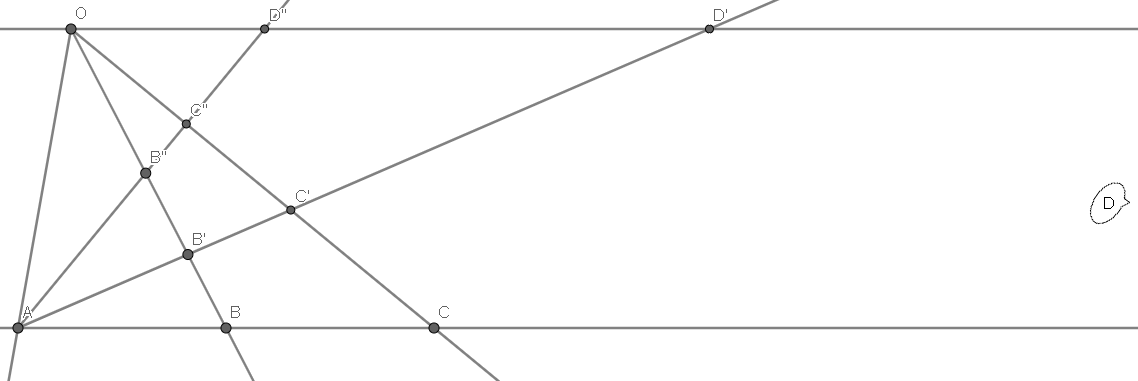
\includegraphics[width=\textwidth]{harmony_at_infinity.png}
\end{figure}
	Hơi khó nhớ, nhưng nếu ta viết: ``nếu $-1 = (AB, C \infty )$ thì $\frac{ \overline{BA}}{ \overline{BC}} = -1$, hay $B$ là trung điểm $AC''$, định lý sẽ dễ nhớ hơn.
	\vskip 0.1cm
	Giải thích cho phát biểu vừa rồi là: khi cho $C$ ngày càng xa khỏi $A$ theo chiều của tia $AB$ thì $(AB, C)$ sẽ dương và ngày càng gần với $1$, khi $C$ ``tại điểm xa vô cùng'' thì cho tỷ số đơn đó bằng $1$ là việc hợp lý, nên ta quy ước $(AB, \infty) = 1$. Khi cho $C$ chạy theo chiều tia $BA$ xa khỏi $B$ thì thu được kết quả y hệt. Nên ta hiểu điểm ``vô cùng'' (nếu có) ở hai đầu đường thẳng là một. Định lý trên không phải trường hợp duy nhất mà sẽ được đơn giản hóa khi thêm vào điểm ``vô cùng'': chẳng hạn như định lý Pascal và Desargues có thể bớt đoạn ``hoặc đôi $1$ song song'' trong kết luận, vì có thể quy ước giao điểm của các đường song song khi này là điểm ở xa vô cùng, giống như cách hai đường ray song song khi kéo dài ra chân trời sẽ tạo cảm giác như là chúng cắt nhau.
	\vskip 0.1cm
	
\textbf{Hiệp bổ sung:}

\begin{figure}[ht]
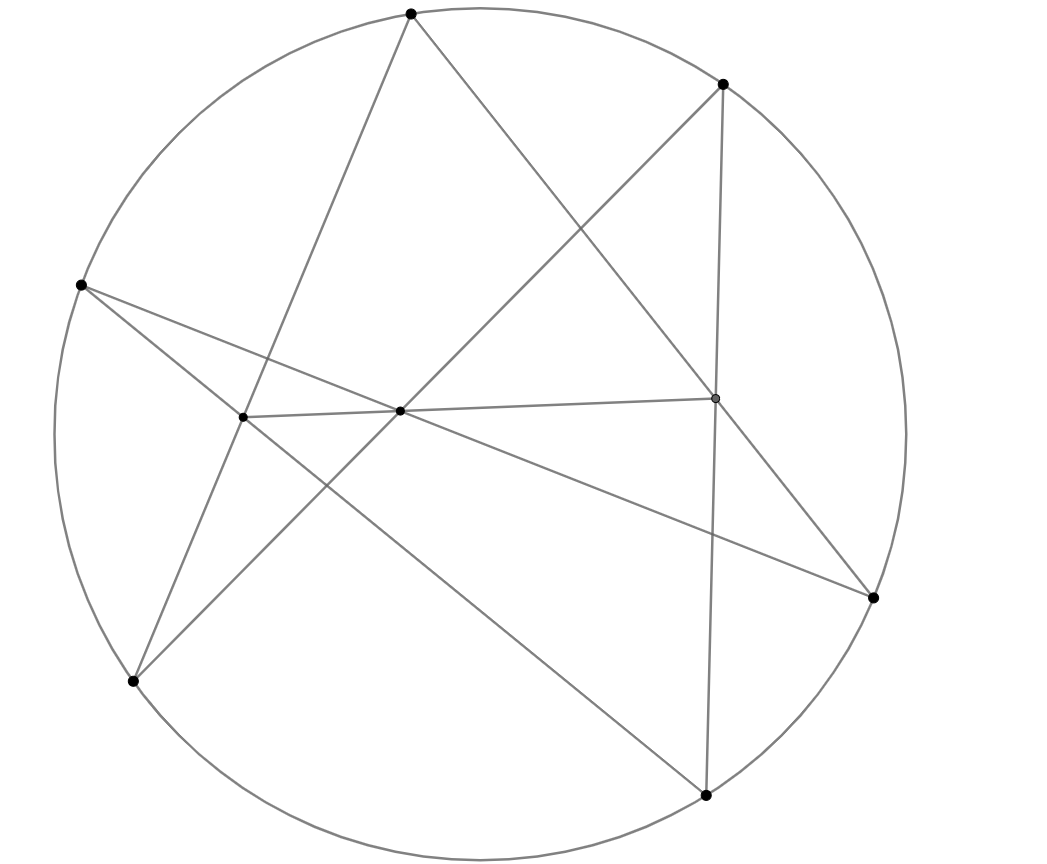
\includegraphics[width=\textwidth]{Pascal_theorem.png}
\end{figure}
\caption: 
(Lục giác huyền bí của cậu thiếu niên Blaise Pascal 17 tuổi, tổng quát hóa hơn 400 định lý hình học từ thời cổ đại đến lúc ấy. Chứng minh bằng tỷ số kép sẽ bao quát được mọi thế hình và các trường hợp suy biến.)	
		\vskip 0.1cm
	Dựa trên sự thuận tiện ấy, ta sẽ quy ước những đường thẳng cùng song song với một đường thẳng $l$ cho trước thì cùng đi qua một điểm gọi là điểm vô cùng ứng với $l$. Hai đường có chung điểm vô cùng khi và chỉ khi chúng song song hoặc trùng nhau. Để Tiên đề $1$ về NTĐQ đã nêu trên không bị vi phạm, ta cần thêm một đường thẳng ``ở vô cùng'' mà đi qua tất cả và chỉ những điểm vô cùng. Sau khi thêm vào mặt phẳng Euclid thông thường những điểm này, ta được một mặt phẳng mà các tiên đề NTĐQ của ta vẫn đúng và có tính chất elliptic. Ta gọi đây là một mặt phẳng xạ ảnh.
	\vskip 0.1cm
	Xét một điểm $N$ không phải điểm vô cùng trên mặt phẳng ấy, vẽ một mặt cầu tâm $O$ tiếp xúc mặt phẳng vừa xây dựng tại $N$. Với mỗi điểm $M$ trên mặt phẳng, biến $M$ thành giao điểm của $OM$ với bán cầu chứa $N$ của mặt cầu. Riêng với điểm vô cùng, do khi một điểm đi dọc một đường đi qua $N$ ra xa khỏi $N$ theo hai phía thì ảnh của nó tiến dần tới hai điểm đối xứng nhau qua $O$, mà đường thẳng lại chỉ có $1$ điểm vô cùng , ta sẽ quy ước hai điểm đối xứng nhau qua $O$ như là $1$ điểm. Và thế là ta được một mô hình khác cho một không gian mà tiên đề song song của hình elliptic đúng và tuân thủ các tiên đề về ``nằm trên đi qua'' đã nêu. Tất nhiên không gian này còn thiếu những khái niệm góc, độ dài cạnh, diện tích, nhưng tạm thời thế đã.
	\begin{figure}[H]
		\vspace*{-5pt}
		\centering
		\captionsetup{labelformat= empty, justification=centering}
		\includegraphics[width= 1\linewidth]{Stereographic projection.png}
%		\caption{\small\textit{\color{}}}
		\vspace*{-10pt}
	\end{figure}
	(Khi các điểm ra xa khỏi $N$ theo cùng một hướng thì ảnh của chúng gần lại với một điểm trên xích đạo.)
	
	
Mô hình này chỉ ra rằng: chính hành tinh quê nhà chúng ta sống là một bề mặt nơi mà mọi đường thẳng (ở đây là các đường tròn lớn) đều cắt nhau.

\begin{figure}[ht]
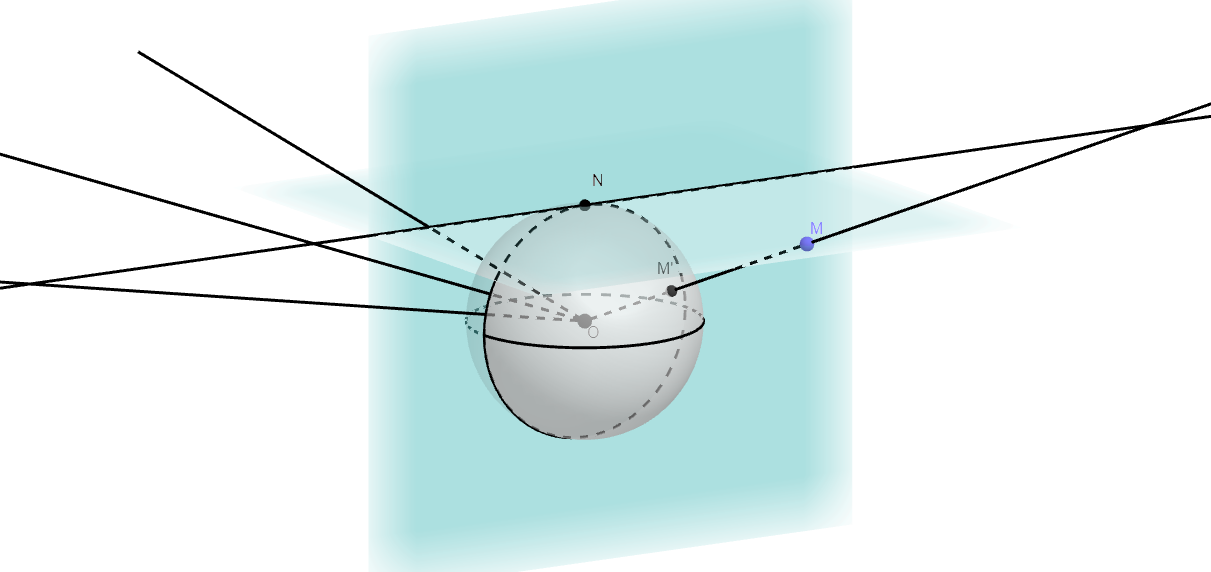
\includegraphics[width=\textwidth]{Stereographic_projection.png}
\end{figure}

(Khi các điểm ra xa khỏi N theo cùng một hướng thì ảnh của chúng gần lại với một điểm trên xích đạo.)

Giờ là lúc đến với một mô hình của hình hyperbolic, mô hình Beltrami-Klein

\section{Mô hình Beltrami-Klein}
Chúng tôi sẽ không trình bày y hệt như công trình gốc của Klein để đỡ phức tạp, nhưng những ý tưởng chủ đạo vẫn là do Klein cải thiện từ luận án của Beltrami.
Cũng giống với hình học Euclid, hình học hyperbolic cũng có mặt phẳng xạ ảnh để hoàn thiện cho không gian hyperbolic thông thường. Dựa vào đó, Klein đã xây dựng mô hình dưới đây từ mặt phẳng đó để nghiên cứu rõ hơn.
Xét một đường tròn $\gamma$ với tâm O và đường kính OR trên mặt phẳng Euclid, gọi phần bên trong của $ \gamma$ là tập hợp các điểm X sao cho OX < OR (tức là không bao gồm điểm nằm trên đường tròn). Một dây cung của đường tròn là một đoạn nối hai điểm trên đường tròn đó.
Trong mô hình Beltrami - Klein, tập hợp các điểm sẽ là phần bên trong của đường tròn, và với mỗi hai điểm A, B từ tập hợp đó, ta định nghĩa ``đường thẳng'' nối A, B là dây cung của $ \gamma$ đi qua AB và bỏ đi hai đầu mút. Ta gọi một dây cung nhu vậy là dây mở và ký hiệu là A)(B. Quan hệ ``nằm trên'' được định nghĩa giống hệt với trong hình học Euclid: P nằm trên A)(B nếu P nằm trên đường thẳng AB theo nghĩa hình Euclid và P nằm giữa A và B. Quan hệ ``nằm giữa'' với hình hyperbolic ở đây là y như quan hệ nằm giữa trong hình Euclid. Quan hệ ``bằng nhau'' sẽ được định nghĩa ở phần tới, do nó phức tạp hơn.
Hình vẽ dưới đây là một minh họa để thấy tiên đề song song của hình hyperbolic đúng trong mô hình này: hai đường qua điểm P không hề có giao điểm với dây kia trong mô hình. Nhìn thì có vẻ hiển nhiên, nhưng riêng việc xét mô hình này đã là một ý tưởng đột phá rồi. 


\begin{figure}[ht]
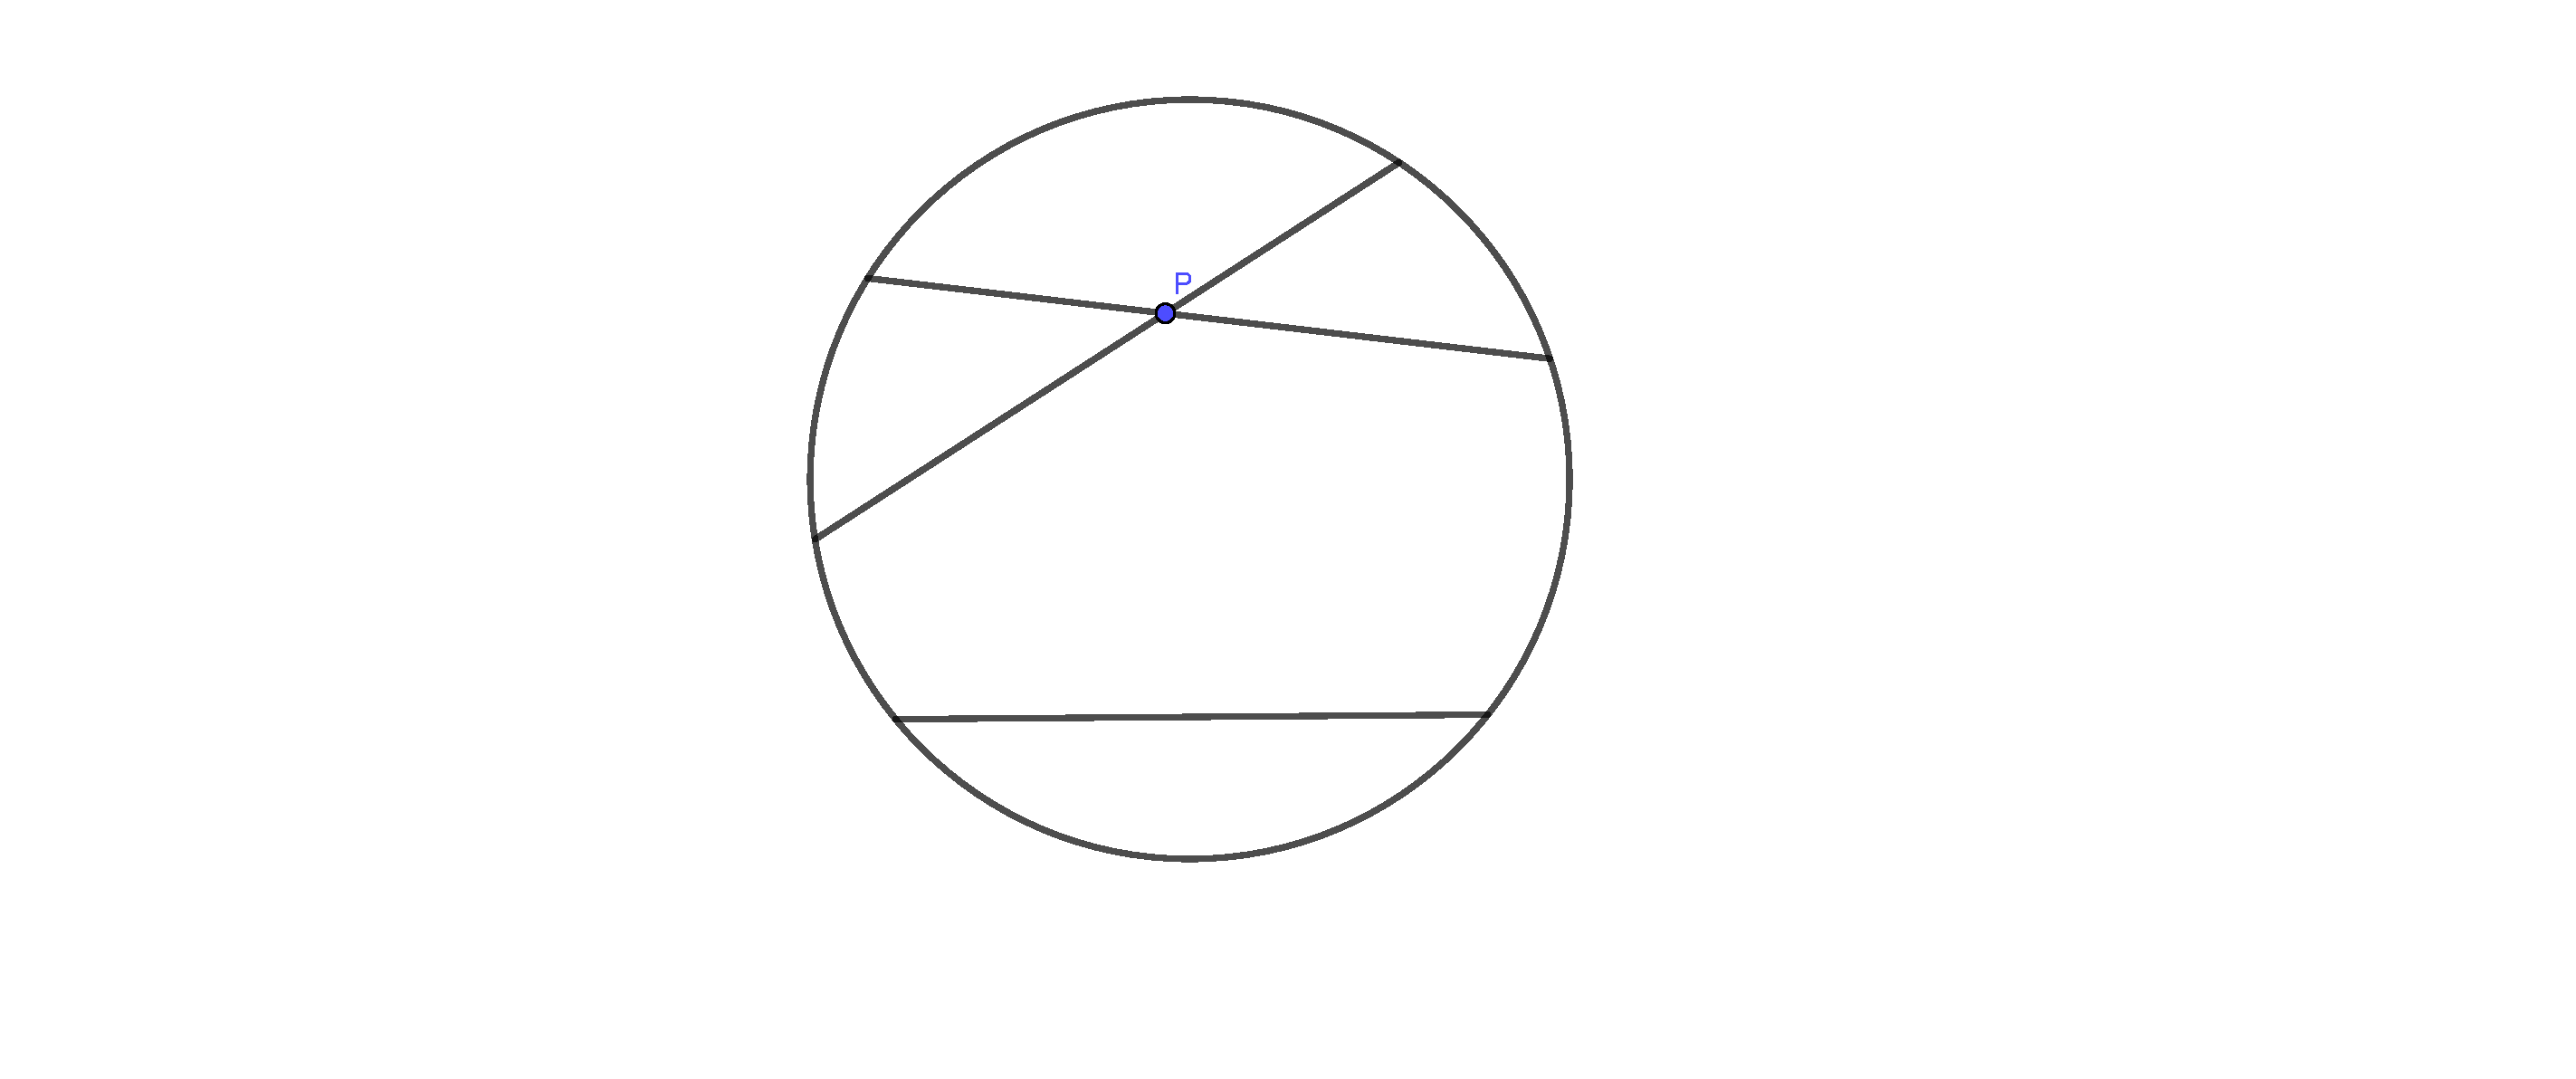
\includegraphics[width=\textwidth]{Hon_mot_duong_song_song.pdf}
\end{figure}


Để chứng minh tính phi mâu thuẫn của hình hyperbolic tương đối với hình Euclid, đầu tiên ta dịch các khái niệm nguyên thủy (``điểm'', ``đường'', ``nằm trên'', ``nằm giữa'' và ``bằng nhau'') trong hình hyperbolic sang một cách diễn giải trong hình Euclid, như cách mà ta đã làm với bốn khái niệm đầu tiên. Các đối tượng có định nghĩa cũng sẽ được dịch sang hình Euclid một cách tương tự. Ví dụ : thay mọi từ ``đường thẳng'' trong phát biểu cho mối quan hệ song song trong hình Euclid thành từ ``dây mở'', và ta thu được định nghĩa cho quan hệ ``song song'' trong hình hyperbolic Sau khi các khái niệm được chuyển đổi xong, ta có thể chuyển sang cắt nghĩa các tiên đề. Chẳng hạn như một tiên đề NTĐQ được dịch về mô hình Beltrami – Klein như sau:\\
Tiên đề NTĐQ 1 (Klein): Với mỗi hai điểm A, B phân biệt ở phần bên trong đường tròn $\gamma$, tồn tại đúng một dây mở l của $\gamma$ sao cho cả A và B nằm trên l. \\

Nhiệm vụ tiếp theo của ta là chỉ ra tiên đề hyperbolic này là một định lý trong hình Euclid, và làm điều này với tất cả các diễn giải tiên đề còn lại. Một khi các tiên đề hình hyperbolic trong mô hình Beltrami – Klein đã trở thành định lý trong hình học Euclid, thì mọi chứng minh là hình học hyperbolic có mâu thuẫn sẽ có nghĩa là một tập hợp các mệnh đề đúng (chính là các tiên đề hình hyperbolic trong mô hình của ta) trong hình Euclid đã dẫn tới mâu thuẫn, từ đó cho thấy một mâu thuẫn trong hình học Euclid. Điều này không thể xảy ra nếu ta giả sử hình Euclid là phi mâu thuẫn.
Quay trở lại, ta vẫn cần chứng minh tiên đề vừa phát biểu kia là một định lý trong hình Euclid.
Thật vậy, gọi l là đường thẳng theo nghĩa trong hình Euclid đi qua A và B. Bởi l có đi qua điểm nào đó nằm trong $\gamma$, nó sẽ có đúng hai giao điểm với $\gamma$, gọi là C và D (Nguyên lý liên tục đường thẳng - đường tròn của hình Euclid). Khi ấy dây mở CD chính là ``đường thẳng'' đi qua A và B, và theo tiên đề NTĐQ của hình Euclid ta có sự tồn tại duy nhất của CD.

Sự tồn tại của  đường song song giới hạn có thể được chỉ ra khá dễ dàng trong mô hình Beltrami-Klein. Nhìn hình ta thấy, hai dây mở (AE) và BF đi qua P chính là hai đường song song giới hạn khi xét đường thẳng là dây mở AB và điểm P không nằm trên đó.

\begin{figure}[ht]
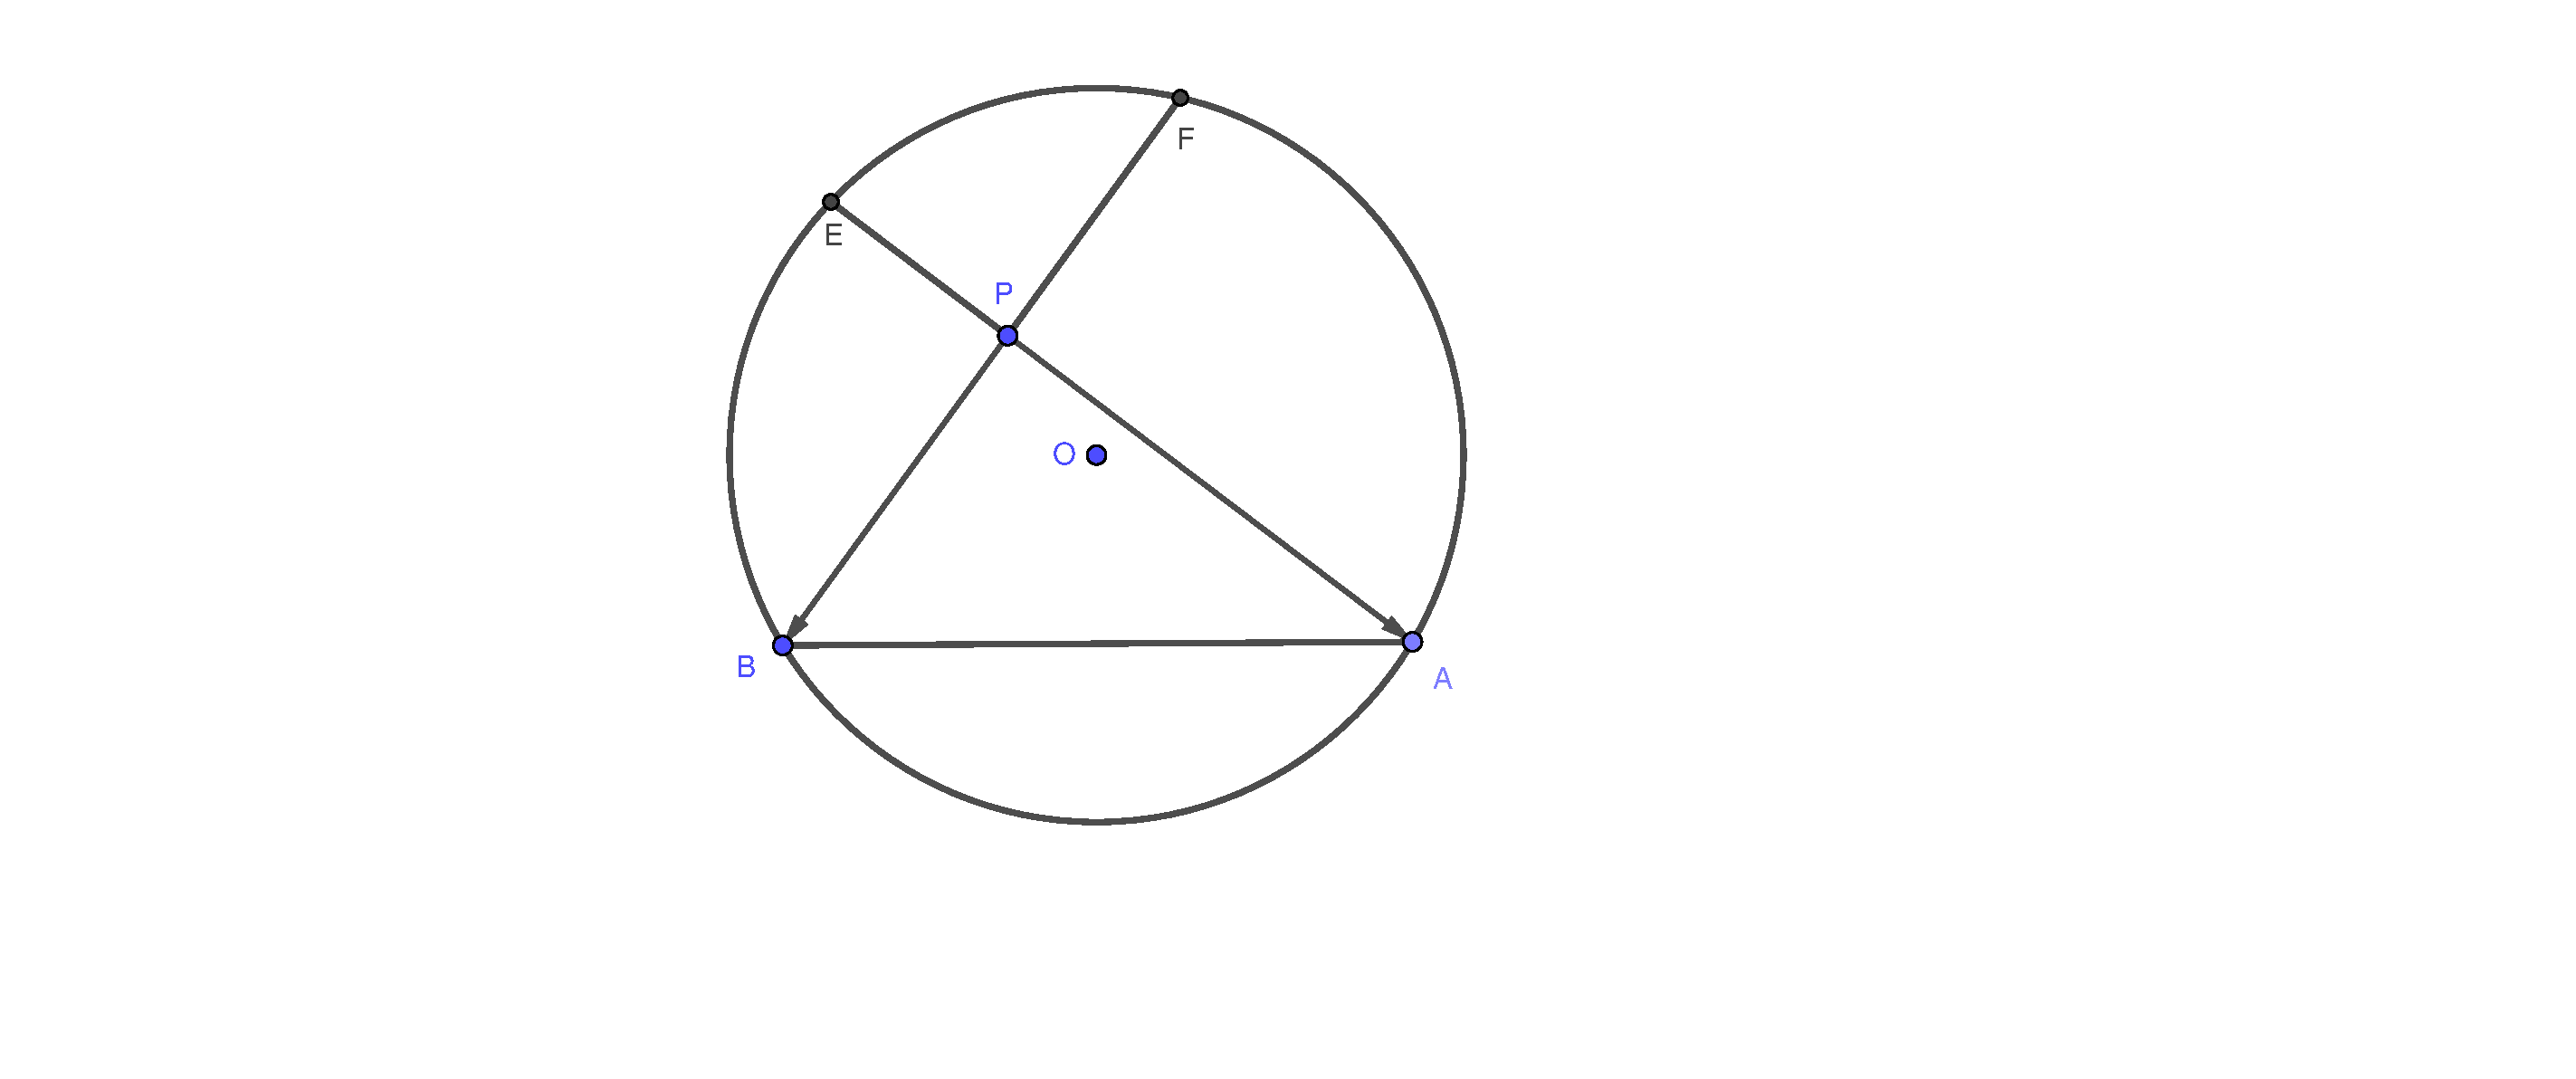
\includegraphics[width=\textwidth]{Duong_song_song_gioi_han_Klein.pdf}
\end{figure}	
	
	
